%# -*- coding: utf-8-unix -*-
%%==================================================
%% chapter01.tex for SJTU Master Thesis
%%==================================================

%\bibliographystyle{sjtu2}%[此处用于每章都生产参考文献]
\chapter{系统设计}
\label{chap:sys_design}

本章首先介绍基于SSD、HDD的混合存储系统的设计动机与设计目标,然后展开描述了系统架构、数据映射策略、冷热数据识别策略、数据写回/迁移策略、最优化存储设备组合等设计。

\section{设计动机与设计目标}

\subsection{设计动机}

在上一章介绍了现在被广泛应用的三种开源混合存储系统flashcache、dm-cache和bcache,他们在性能、可靠性、内存开销等方面都有各自的优点与缺点,但有两个问题是这三个混合存储系统都未解决的。

第一个问题是这三个混合存储系统的最优化存储设备组合,他们都不支持将多存储设备与多后台设备统一为一个逻辑设备供用户使用。flashcache和dm-cache都仅支持单缓存设备对单后台设备,bcache支持单存储设备对多后台设备。对于普通用户而言,单个缓存设备已经足够应付正常的I/O负载,但对服务器级别的I/O负载来说,由于本身存储的数据量大,且I/O负载重,为了保证缓存的高命中率,缓存设备的容量也应相对数据量进行提升,但是如果混合存储系统仅支持单缓存设备,那么就需要单个大容量的缓存设备,成本会急剧上升,而如果混合存储系统支持多缓存设备,就可以以多个小容量的缓存设备实现大缓存容量,降低成本。

另一个问题是这三个混合存储系统都不支持针对不同进程设置不同权限,按权限分配进程的I/O带宽,由于系统整体的I/O带宽有限,在重负载情况下系统可能无法满足全部进程的I/O带宽要求,如果系统只是简单地将总I/O带宽平均分配给所有进程或者以先来先得的策略分配,可能会造成高权限的进程不如低权限进程的情况。为了解决这两个问题,需要设计一套新型混合存储系统,在保证系统的大容量、低成本、高性能的前提下实现对多缓存设备对多后台设备的支持以及对支持按进程权限分配I/O带宽的功能。

\subsection{设计目标}

本混合存储系统的设计目标如下:

\begin{enumerate}
    \item 大容量。系统应具有较大的容量,且应能支持多缓存设备对多后台设备的缓存。
    \item 低成本。系统的存储成本应接近HDD的存储设备。
    \item 高顺序读写性能。系统的顺序读写性能应至少接近HDD的性能。
    \item 高随机读写性能。系统的随机读写性能应接近SSD的性能。
    \item 支持I/O带宽按权限分配。系统应支持按照进程的权限分配不同进程的I/O带宽。

\end{enumerate}

\section{系统架构}

系统总体架构如图\ref{fig:system_architecture}所示。系统首先将缓存设备与后台设备各自虚拟成一个统一的存储空间的虚拟缓存设备和虚拟后台设备进行管理,然后将虚拟缓存设备与虚拟后台设备虚拟为一个设备设备进行统一管理,并提供给用户使用。系统在接收到I/O请求后,通过映射机制将I/O进行分割,然后将分割后的I/O交给缓存管理模块,缓存管理模块首先进行存储地址查找,如果在缓存设备上则直接返回地址,否则进入数据冷热识别,并经缓存替换策略后发起缓存数据的更新操作。虚拟缓存设备和虚拟后台设备在收到请求后也经过存储位置查找,将对数据块的请求交给对应的真实设备处理。

\begin{figure}[!htp]
    \centering
    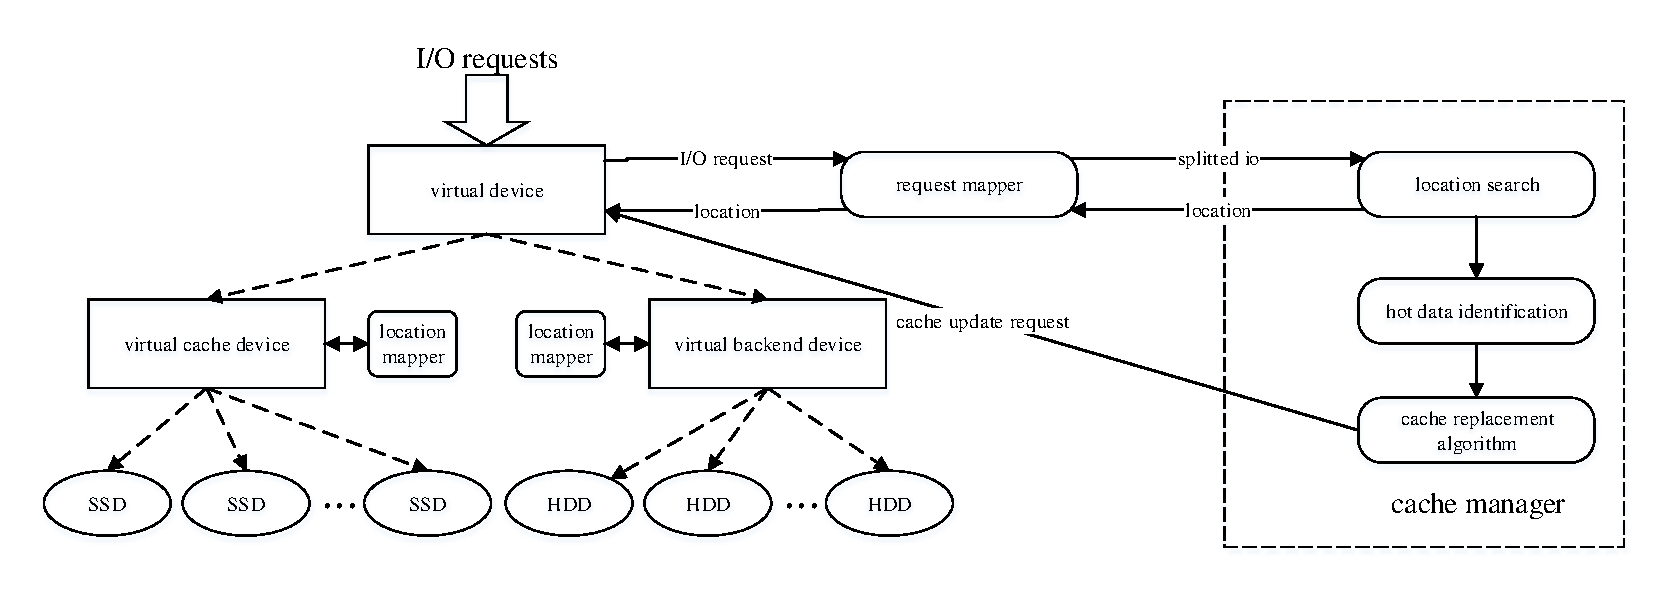
\includegraphics[width=\textwidth]{system_architecture.pdf}
    \bicaption[fig:system_architecture]{系统整体架构}{系统整体架构}{Fig}{overall system architecture}
\end{figure}

系统整体采用分层架构,利用SSD较高的随机读写性能将SSD用作随机I/O缓存,将HDD作为源存储介质存储所有的数据,SSD上存储HDD中数据的子集,系统可用容量等于HDD的总容量。数据的流动规则如图\ref{fig:data_flow}所示,系统将随机I/O请求交由SSD处理,将随机I/O请求交由HDD处理,SSD与HDD之间进行数据的交换,HDD将热数据写入到SSD中提高系统整体的性能,SSD将被替换的数据写回到HDD中保证系统的一致性。

\begin{figure}[!htp]
    \centering
    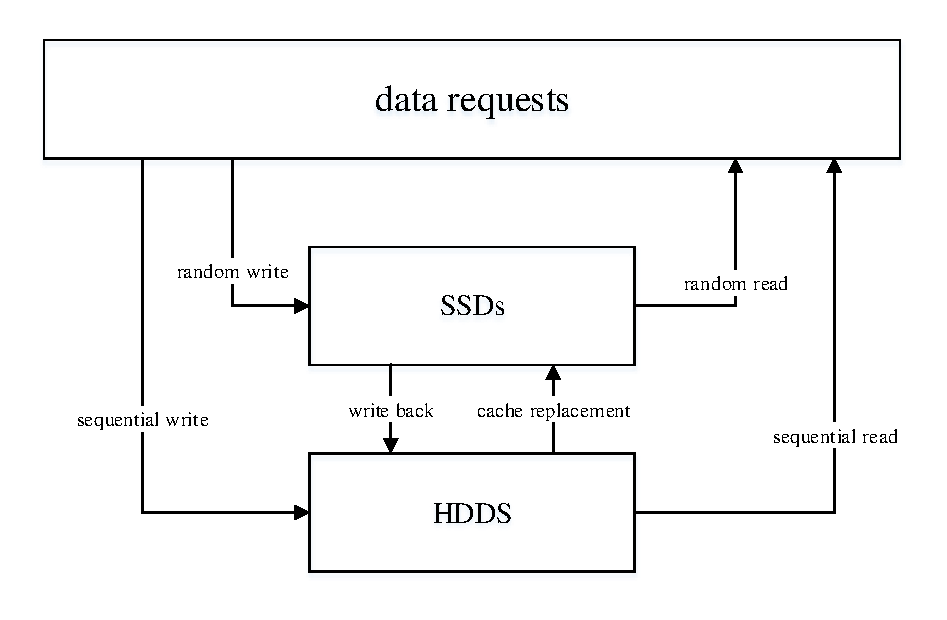
\includegraphics[width=0.8\textwidth]{data_flow.pdf}
    \bicaption[fig:data_flow]{数据流示意图}{数据流示意图}{Fig}{data flow}
\end{figure}

\section{数据映射策略}
TODO,与flashcache相同。

\section{冷热数据识别策略}

TODO,与flashcache相同。

\section{数据写回/迁移策略}

TODO,与flashcache相同。

\section{最优化存储设备组合}

在系统架构中可以看到,本系统对于多缓存设备和多后台设备的管理采用增加一层虚拟层的策略。系统不直接将多个缓存设备和多个后台设备统一为一个虚拟设备进行管理以供用户使用,而是首先将多个缓存设备统一成一个虚拟缓存设备,将多个后台设备统一成一个虚拟后台设备。

分层管理通过增加中间层,相比直接管理多个设备,系统可以将设备管理策略与系统架构、数据映射策略、冷热数据识别策略、数据写回/迁移策略等缓存策略隔离开,使策略的配置更简单。例如,如果要保证多个缓存设备的容量被均衡地使用,在直接管理下,相应的数据映射策略和数据写回/迁移策略都要对应修改,但在分层管理下,数据映射策略和数据写回/迁移策略可以维持不变,只需要改变设备管理策略,将多个设备以raid0生成对应虚拟设备即可。如果要保证数据的可靠性,配置多副本,则在直接管理下,需要将设备分组管理、分组操作,对应的各种操作都需要改变,而在分层管理下只需要以raid1配置设备即可。

分层管理虽然在策略配置上更灵活,但相比直接管理,系统在扩容上会略显不足。在直接管理下,对系统的扩容可以实现热扩容,即在系统运行的状态直接进行扩容操作,直接增加被管理的设备并更新对应的参数变化即可。与之相对,在分层管理下,由于设备管理与其它部分隔离,为了保证扩容后系统的正确性,需要先将虚拟缓存设备的数据全部写回虚拟后台设备,然后禁用缓存,对系统进行扩容,再开启缓存,系统整体会有性能下降的一段时间,且影响时间与被缓存的数据量有关,即约与虚拟缓存设备的容量成正比。

本文的研究认为,对于普通用户而言,系统基本不存在扩容这一行为,而对于服务器级用户而言,扩容也并不是一种经常进行的行为,但是对于设备管理策略的变更的频率确是相对而言比较高的。设备管理的策略主要与系统的I/O负载类型有关,变化比较多样,有的可能只是要求设备负载均衡,有的可能只是要求能提供灾备,但有的可能会很复杂,是多种简单策略的组合。如果采用直接管理的模式,虽然也能实现各种策略,但是对应的代码修改量会十分巨大,分层管理则可利用现有的技术如LVM\cite{wada2009logical}完成。

\section{I/O带宽按权限分配}

系统通过对不同进程按照各自权限分配IOPS来限制不同进程的I/O带宽,采用CFQ(Completely Fair Queuing)策略,如图\ref{fig:system_io_scheduler}所示,每个进程都被分配一个队列,每个I/O请求被放到对应进程的队列中,根据每个进程的权限不同,给每个进程的I/O请求分配不同的时间片数量,每个时间片取出I/O请求通过映射到实际设备进行请求处理。

\begin{figure}[!htp]
    \centering
    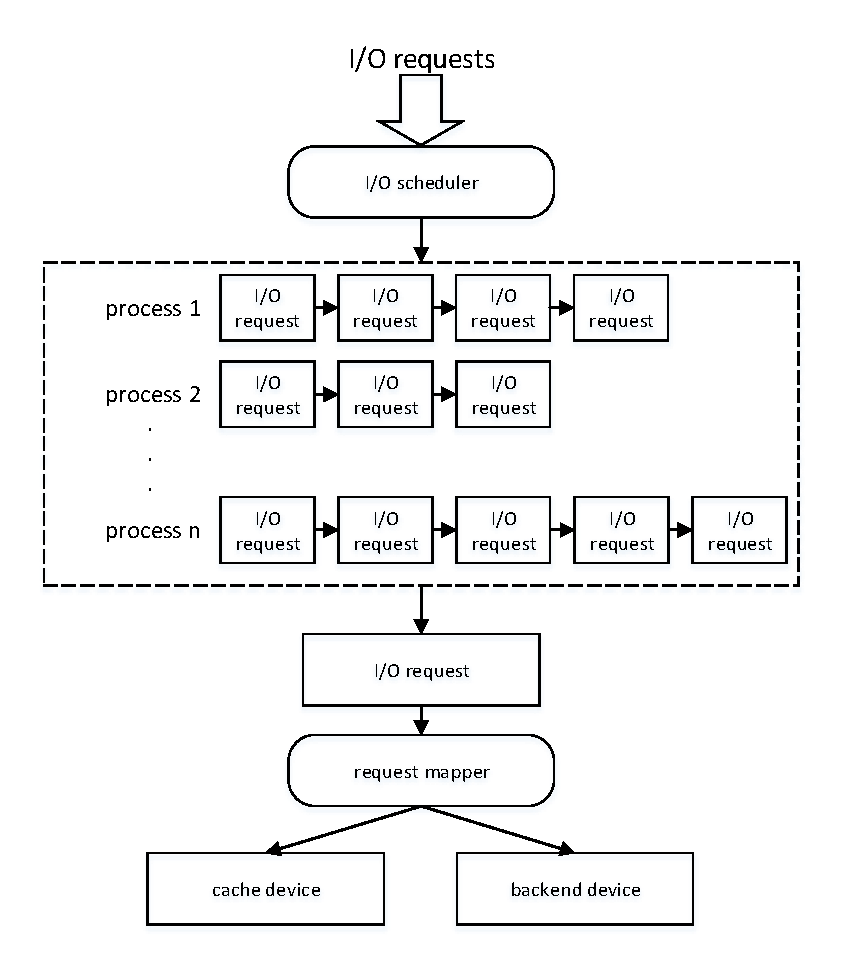
\includegraphics[width=0.8\textwidth]{system_io_scheduler.pdf}
    \bicaption[fig:system_io_scheduler]{I/O带宽分配流程}{I/O带宽分配流程}{Fig}{I/O bandwidth quota process}
\end{figure}

\section{本章小结}

本章介绍了系统在设计过程中所遇到的问题以及对分析与解决思路。介绍了系统的设计动机与设计目的,并对优化存储设备组合与I/O带宽按权限分配等问题的策略选择进行了分析,为接下来的系统实现做准备。